\chapter{Grundlagen medizinischer Daten- und Bildformate} \label{grundlagen}
\addthumb{Grundlagen der medizinischen Bildverarbeitung}{\huge{\textbf{\thechapter.}}}{white}{haw_rot}

\section{Bildgewinnung und bildgebende Verfahren}\label{grundlagen:bildgebung}

\section{DICOM}\label{grundlagen:dicom}
Der Name DICOM steht für \textit{Digital Imaging and COmmunication in Medicine}. Der Umgang mit diesem Standard ist essentieller Bestandteil der zu entwickelnden Software. Pianykh\cite{pianykh:dicom} beschreibt im ersten Kapitel, dass DICOM nicht nur aus Pixel und deren zugehörigen Werten besteht. Wie der Name sagt, ist auch die Kommunikation fest im Standard verankert. Damit ist die Übertragung der Daten von medizinischen Geräten(Modalitäten) zum zentralen Speicher und deren Verteilung gemeint. Des weiteren spielt die dauerhafte Speicherung der digitalen Aufnahmen eine große Rolle. Daher wird im gleichen Zug mit DICOM immer ein PACS genannt. Das Akronym PACS bedeutet \textit{Picture Archiving and Communication System} und besteht sowohl aus Hardware (Server, Speicherung) als auch Software(Verteilung und Kommunikation).\\
Abbildung \ref{communication} illustriert das Zusammenspiel des DICOM-Standards und dem zentralen Datenspeicher. Zuerst wird mittels der Modalitäten(z.B. mit dem Computertomographen oder einem Ultraschallgerät) die digitale Aufnahme erzeugt. Danach wird das Bild vom Gerät an das PACS gesendet. Hier werden die Aufnahmen und Patientendetails in die Datenbank und den Speicher abgelegt. Wird eine Aufnahme benötigt können Clients Anfragen mit beispielsweise dem Patientennamen stellen und erhalten die zugehörige Serie mit der digitalen Aufnahme.

\begin{figure}[htbp]
  \vspace{0.5cm}
  \centering
  \fbox{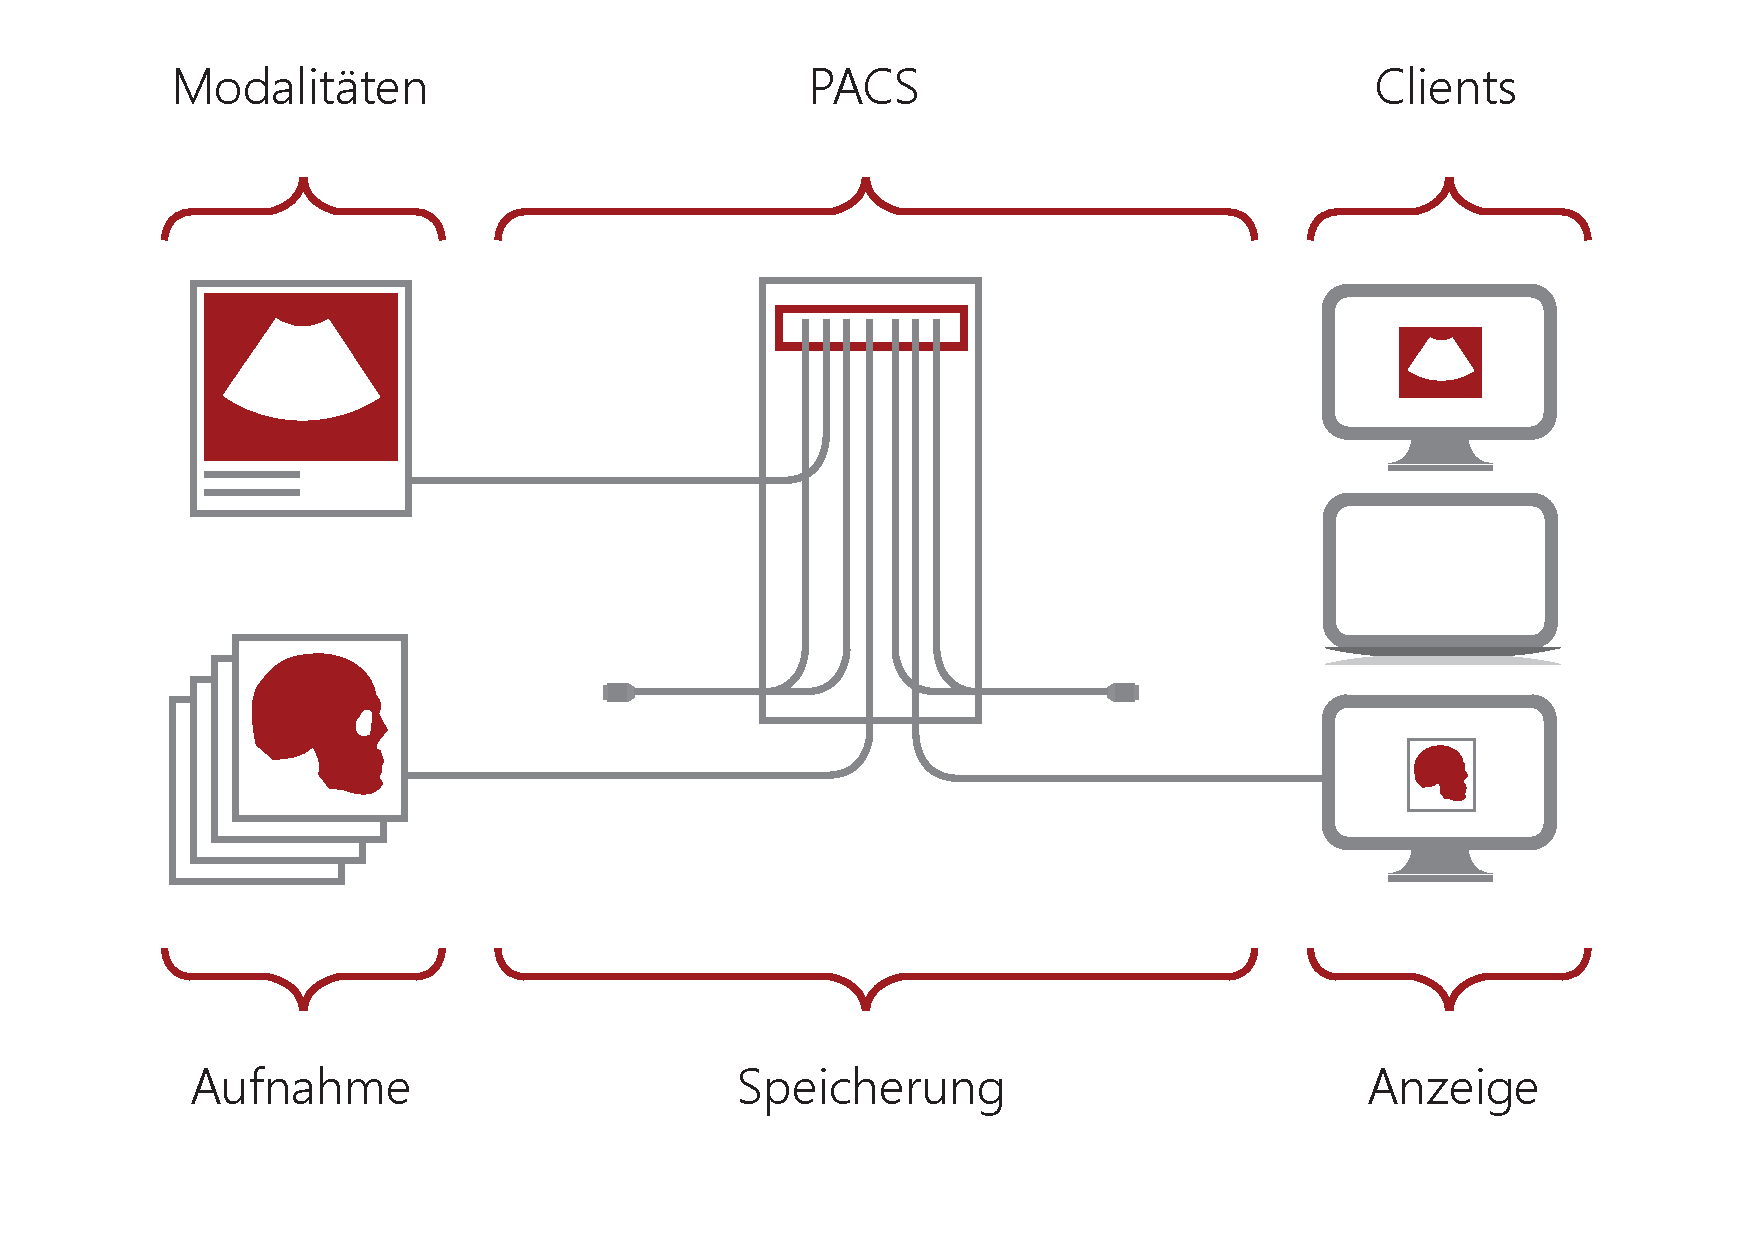
\includegraphics[angle=0,width=12cm]{./img/communication_neu.pdf}}
  \caption{Kommunikationsprozess von Aufnahme zur Verarbeitung}
  \floatfoot{Vorlage für diese Darstellung ist die Grafik in \cite[Fig. 1]{pianykh:dicom}}
  \label{communication}
  \vspace{0.5cm}
\end{figure}

DICOM\footnote{Unter ftp://medical.nema.org/medical/dicom/ lässt sich der aktuelle Standard abrufen. Die Kapitel befinden sich im Ordner zum jeweiligen Jahr der Veröffentlichung. Aktuell sind die Dokumente von 2011.} ist daher nicht nur ein einzelner Standard, sondern verknüpft die standardisierte 
\begin{itemize}
\item Kommunikation,
\item Erzeugung der Bilddaten,
\item und Speicherung.
\end{itemize}
Im Rahmen dieser Abschlussarbeit liegt der Fokus auf den Bilddaten, daher wird auf die Kommunikation- und Speicheraspekte nicht im Detail eingegangen.

\subsection{Die Dicom Information Object Definitionen} \label{grundlagen:iod}
Bevor die Pixeldaten genauer betrachtet werden können, muss der prinzipielle Aufbau der Dicomobjekte beschrieben werden. Teil 3 des Standards\cite[A.1.2]{dicom:iod} zeigt den relationalen Aufbau der Dicomobjekte. Vereinfacht können die elementaren Informationsobjekte in drei Teile aufgeteilt werden.

\begin{itemize}
	\item \textbf{Patient}\\
	Der Patient steht in der Hierarchie an oberster Stelle und ist die Grundlage für eine oder mehrere Studien(Study).
	\item	\textbf{Study}\\
	Study symbolisiert eine medizinische Studie. Eine Studie ist eine Sammlung von mehreren Serien, die von Modalitäten wie CT und MR aufgezeichnet werden. Eine Studie ist exakt einem Patient zugeordnet.
	\item \textbf{Series}\\
	Eine Serie ist ein Folge von Bildern, die von einer Modalität erzeugt wird. Die Aufnahmen eines CT werden einer Serie zugeordnet. Jede Serie gehört zu nur einer Studie.
	\item \textbf{Image, Real World Values}\\
	Auf der unteren Hierarchiestufe stehen Objekte wie Bilddaten oder die Lage des Patienten im Raum während der Aufnahme. Ein Bild wird genau einer Serie zugeordnet.
\end{itemize}

Aus diesen vier elementaren Objekten ergibt sich folgende Informationsstruktur für Dicomobjekte, die in Abbildung \ref{ermodel} als Entity-Relationship-Modell\footnote{Ein ER-Modell beschreibt die Beziehungen der Elemente zueinander. Dieser Diagrammtyp wird unter Anderem häufig beim Entwickeln der Struktur einer relationalen Datenbank verwendet} verdeutlicht wird.

\begin{figure}[htbp]
  \vspace{0.5cm}
  \centering
  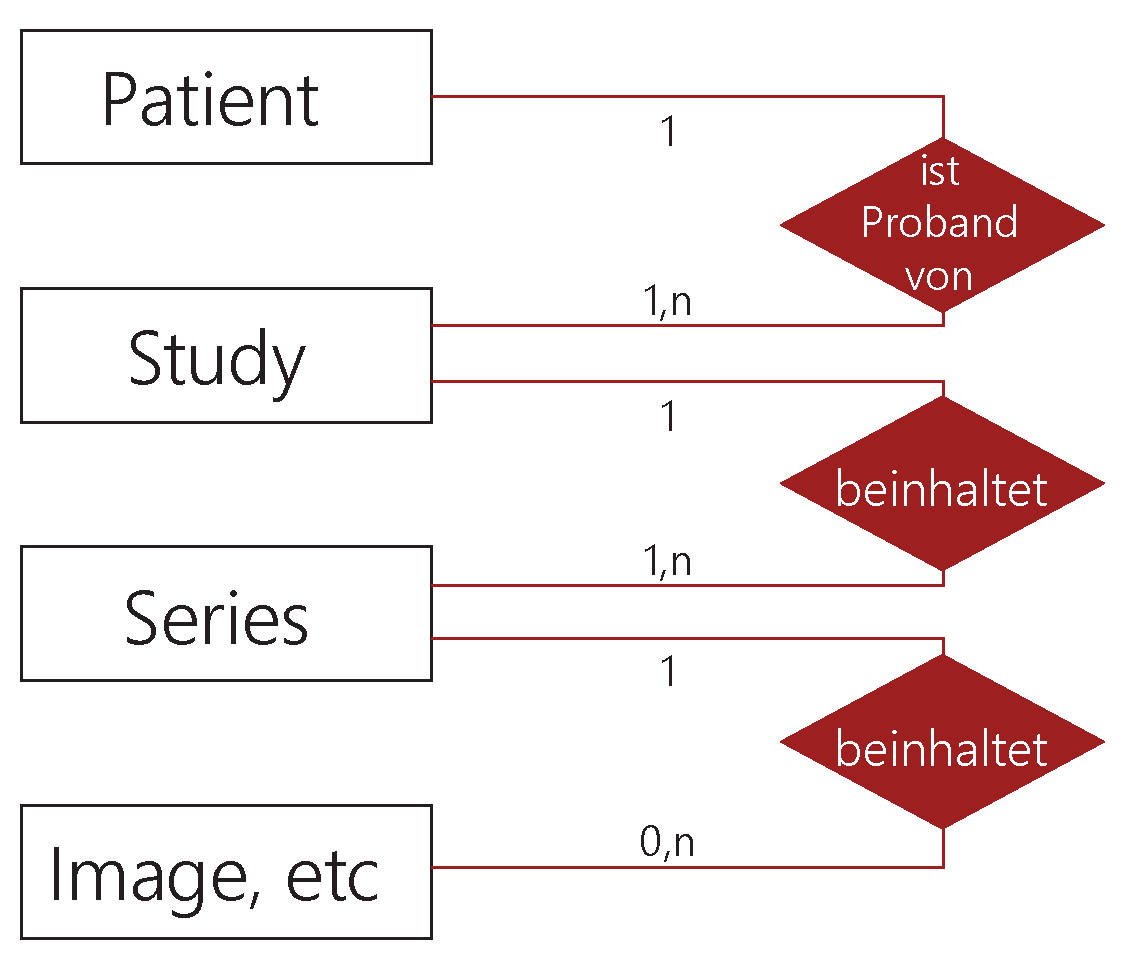
\includegraphics[angle=0,width=8cm]{./img/ermodel.pdf}
  \floatfoot{Vorlage für diese Darstellung ist die Grafik in \cite[A.1.2]{dicom:iod}}
  \caption{Vereinfachte Darstellung der Informationsobjekthierarchie von Dicomelementen}
  \label{ermodel}
  \vspace{0.5cm}
\end{figure}

Der DICOM-Viewer OsiriX bietet auf der Herstellerseite\footnote{http://www.osirix-viewer.com/datasets/} die Möglichkeit Testdaten zu beziehen. Betrachtet man die Repräsentation der Daten auf der Festplatte hält sich die Ordnerstruktur an obiges ER-Modell.\\
Abbildung \ref{filesystemrep} zeigt eine schematische Darstellung der Dateien. Die Beispieldaten von OsiriX bestehen aus einem Patient names \glqq Brebix\grqq\, dem eine Studie sowie zwei Serien à 100 Aufnahmen zugeordnet werden.

\tikzstyle{every node}=[draw=black,thick,anchor=west]
%\tikzstyle{selected}=[draw=red,fill=red!30]
\tikzstyle{optional}=[dashed,fill=gray!50]
\begin{figure}[htbp]
\centering
\caption{Repräsentation der Information Objekte im Dateisystem}
\label{filesystemrep}
\begin{tikzpicture}[%
  grow via three points={one child at (0.5,-0.7) and
  two children at (0.5,-0.7) and (0.5,-1.4)},
  edge from parent path={(\tikzparentnode.south) |- (\tikzchildnode.west)}]
  \node {Dicom Ordner}
    child [missing] {}
    child { node {BREBIX - Patient}
    	child [missing] {}
    	child { node{CT10 ponction foie - Studie}
    		child [missing] {}
    		child { node {DEF FOIE ART. - 107198 - Serie}
    			child{node[optional]{IM-0001-0001.dcm}}
    			child{node[optional]{...}}
    			child{node[optional]{IM-0001-0100.dcm}}
    		}
    		child [missing] {}				
    		child [missing] {}				
    		child [missing] {}
    		child [missing] {}
    		child { node {DEF. VEINEUX - 107205 - Serie}
    		    child{node[optional]{IM-0001-0001.dcm}}
    		    child{node[optional]{...}}
    		    child{node[optional]{IM-0001-0100.dcm}}
    		}
    		child [missing] {}
    	}
    };		
\end{tikzpicture}
\end{figure}

Bei näherem Hinsehen fällt auf, dass die Dateinamen beider Serien des Patienten identisch sind. Eine korrekte Zuordnung von DICOM-Dateien zur Serie ist daher nicht immer garantiert. Unabhängig von einer Repräsentation im Dateisystem oder Pfadangaben in der Datenbank eines PACS ist das Vertrauen auf Dateipfade unsicher, da über eine einfache Dateimanipulation die Zuordnung nicht mehr hergestellt werden kann.\\
Um eine zuverlässige Verknüpfung zu gewährleisten besitzt jeder Patient\footnote{Die Identifikationsnummern von Patienten sind meist nur innerhalb einer Institution oder Krankenhauses einzigartig, da diese manuell vergeben werden können\cite[5.6.2]{pianykh:dicom}.}, jede Studie und jede Serie eine Eindeutige Identifikationsnummer. Diese Art der Informationen wird in den einzelnen Dateien mit Hilfe von Einträgen aus dem DICOM Data Dictionary\cite{dicom:dd} hinterlegt. Die DICOM-Dateien beschreibt Pianykh \cite[S. 47]{pianykh:dicom}
als eine Kopie im Speicher vom tatsächlichen DICOM-Objekt.

\subsection{Der Transfer vom Patienten zu digitalen Dicomobjekten} \label{grundlagen:dicomObjects}
Wie der Name bereits andeutet ist das DICOM Data Dictionary vergleichbar mit einem Wörterbuch. Es enthält alle gültigen Elemente, die zur Beschreibung eines DICOM-Objekts verwendet werden können. Zusätzlich zu dem aus dem Standard bekannten Vokabular können Hersteller medizinischer Geräte ein eigenes Dictionary hinzufügen. Die proprietären Elemente können allerdings nicht standardisiert verarbeitet werden(vgl. \cite[S.45]{pianykh:dicom}, da Software die diese Objekte verarbeitet, nichts von der Existenz dieser Elemente weiß).\\
Mit Hilfe des Wörterbuchs und den ca. 2000 enthaltenen Daten können nun Aussagen des wirklichen Lebens (vorausgesetzt die Aussage ist mit einem Element aus dem Wörterbuch darstellbar) ins Digital übersetzt werden.\\
Tabelle \ref{table:patientname} zeigt das DICOM-Element für den Namen des Patienten aus dem Data Dictionary\cite[S. 14]{dicom:dd}.

\begin{table}
    \begin{tabularx}{\textwidth}{|X|X|X|X|X|}
    \toprule
    \hline
    \textbf{Tag}         & \textbf{Tagname}     & \textbf{VR} & \textbf{Wert}     	& \textbf{VM} \\ \hline
    (0010,0010) 		 & PatientName 			& PN 		  & John\^{}Doe 		& 1  \\  \hline
    \bottomrule
    \end{tabularx}
    \caption {Repräsentation des Patientennamen als DICOM-Element}
    \label{table:patientname}
\end{table}

Betrachtet man den folgenden Satz(vgl. \cite[S.46]{pianykh:dicom}), kann dieser in ein DICOM-Object, wie es Tabelle \ref*{table:translation} darstellt, übersetzt werden:
\begin{center}
\textit{\glqq John Doe, männlich, geboren am 01. Januar 1970\grqq}
\end{center}

Aus den Beispielen von Tabelle \ref{table:patientname} und \ref{table:translation} lässt sich erkennen, dass ein DICOM-Element nochmals in atomare Teile aufgespalten werden kann. Folglich besteht ein Datenelement aus einem beschreibenden \textit{Tag}, einer \textit{VR(Value Representation)}, einem Wert und der \textit{VR (Value Multiplicity)}. Das Element selbst nimmt eine von drei Darstellungsmöglichkeiten ein. Zusätzlich liegt im Speicherabbild des Datenelements die Länge des Wertes\footnote{John\^{}Doe besitzt aufgrund der Zeichenmenge eine Länge von acht}. Abhängig von der Transfersytax\footnote{Unter der Transfersystax verstehn man eine Menge an Kodierungsvorschriften von DICOM-Objekten\cite[S.63 Section 10]{dicom:structure}. Zu diesen Vorschriften gehört zum Beispiel die Reihenfolge der Bytes im DICOM-Element oder die Komprimierung der Bilddaten} des DICOM-Objekts ist der VR-Teil optional. Die weiteren beiden Darstellungen unterscheiden sich in der Kodierung der benötigten Länge des Werts \cite[7.1]{dicom:structure}.  Anhang \ref{appendix:speicher} auf Seite \pageref{appendix:speicher} zeigt wie Datenelemente im Speicher abgelegt werden und wie viel Speicherplatz pro Element reserviert werden muss.

\begin{table}
    \begin{tabularx}{\textwidth}{|p{4cm}|p{4cm}|X|X|X|}
    \toprule
    \hline
    \textbf{Tag\newline \small{(Gruppe, Element)}}         & \textbf{Tagname}     & \textbf{VR} & \textbf{Wert}     	& \textbf{VM} \\ \hline
    (0010,0010) 		 & PatientName 			& PN 		  & John\^{}Doe 		& 1  \\ \hline
    (0010,0030) 		 & PatientBirthDate		& DA 		  & 19700101	 		& 1  \\ \hline
    (0010,0040)			 & PatientSex 			& CS 		  & M			 		& 1  \\ \hline
    (0010,1010) 		 & PatientAge 			& AS 		  & 44			 		& 1  \\ \hline
    \bottomrule
    \end{tabularx}
    \caption {Das erzeugte DICOM-Objekt mit den Elementen zu Patientenname, Geburtsdatum, Geschlecht und Alter}
    \label{table:translation}
\end{table}

\subsection{Tags in Datenelementen}

Ein DICOM-Element wie PatientName kann über ein Tag identifiziert werden. Ein Tag ist in einem DICOM-Objekt einzigartig und darf nur ein mal benutzt werden. Die numerische Darstellung hat die Form (\textit{gggg}, \textit{eeee}) wobei die hexadezimalen Ziffern \textit{g} die Gruppe des DICOM-Elements beschreiben und \textit{e} das Element der Gruppe \textit{g} definiert. Zusätzlich zu diesen Eigenschaften, kann bestimmt werden, ob der Ursprung eines DICOM-Elements im Standard- oder einem privaten Data Dictionary liegt. Eine gerade Gruppen-Ziffer zeigt, dass das Element Teil des Standards ist während ungerade für proprietäre Elemente stehen\footnote{Ausgenommen aus dieser Regel sind folgende Gruppen: (0000, eeee), (0002, eeee), (0004, eeee), (0006, eeee), (0001, eeee), (0003, eeee), (0005, eeee), (0007, eeee), (FFFF, eeee)}\cite[7.1]{dicom:structure}. Die Reihenfolge der Tags ist in numerischer Folge in aufsteigender Form sortiert. Fällt während des Einleseprozesses in eine Datei auf, dass die Reihenfolge nicht korrekt ist, deutet dies auf ein korruptes DICOM-Objekt hin.\\

\subsection{VR - Value Representation}
Dieser Teil eines DICOM-Elements beschreibt den Typ und das Format des Wertes\cite[6.2]{dicom:structure}. Der Umfang an verschiedenen Value Representations reicht von Zeichenketten wie PersonName (PN) im Datenelement (0010,0010) PatientName über Datumsangaben (DA) bis zu numerischen Werten(FL) und Sequenzen (SQ). Eine vollständige Liste ist im Standard unter \cite[Table 6.2.1]{dicom:structure} zu finden.\\
Zwecks Vollständigkeit soll erwähnt werden, dass ein Datenelement mit VR-Typ SQ wiederum ein DICOM-Object enthalten kann und dadurch eine Baumstruktur entsteht.

\subsection{VM - Value Multiplicity}
Value Multiplicity bestimmt die Anzahl an Werten, die in einem DICOM-Element enthalten sind. Die Werte werden durch einen Backslash \textbackslash voneinander getrennt. Der explizite Wert der Value Multiplicity kann aus dem Data Dictionary entnommen werden.\cite[6.4]{dicom:structure}

\section{DICOM Pixeldaten und Bildformate}

Die Abschnitte \ref{grundlagen} - \ref{grundlagen:dicomObjects} zeigen, dass DICOM mehr als ein Bildformat darstellt, ein essentieller Bestandteil bleiben jedoch die Pixel eines DICOM-Objekts (auch wenn diese nur optional vorhanden sein müssen, wie Grafik \ref{ermodel} zeigt). Nach dem DICOM Data Dictionary gehören Bild-abhängige Informationen zur Gruppe (\textit{0028}, \textit{eeee}).
Die Pixeldaten liegen im Bereich (\textit{7fe0}, \textit{0010}) am Ende eines DICOM-Objekts.\\
Das bedeutet, dass die konkreten Werte der Pixel im gleichen DICOM-Objekt liegen und den selben Kodierungsrichtlinien der DICOM-Tags unterliegen.

\subsection{Kodierung der Pixel im Speicherabbild eine DICOM-Objekts} \label{pixelkodierung}

Um die grundlegende Struktur der Pixel im DICOM-Objekt zu beschreiben sind drei Datenelemente notwendig: BitsAllocated, BitsStored und HighBit\ref{table:digitalRep}. BitsAllocated beschreibt, wie viel Speicher für einen singulären Pixelwert reserviert wird. Mit Hilfe von Columns und Rows kann die Bilddimension bestimmt werden. Columns beschreibt die Breite, Rows die Höhe. Die Value Representation des Datenelements PixelData (\textit{7fe0}, \textit{0010}) kann nach DICOM Data Dictionary entweder den Wert \textit{OB} oder \textit{OW} annehmen. OB bedeutet \textit{Other Byte String} während OW für \textit{Other Word String} steht. Nach Section 8.1 des Standards\cite{dicom:structure} besteht der Unterschied zwischen den beiden VRs darin, dass OB abhängig von der Byteordnung ist. Ob die Ordnung Little Endian oder Big Endian entspricht ist abhängig von der Transfersyntax des DICOM-Objekts.
Grafik \ref{byteorder} zeigt die Kodierungsreihenfolge. Little Endian kodiert vom Least Significant Bit (LSB) zum Most Significant Bit (MSB). Big Endian verarbeitet die Byte in umgekehrter Reihenfolge. Ein Element von PixelData (sowohl mit einer VR von OB als auch OW) fasst 16 Bit, was gleichzeitig die maximale Größe an allokiertem Speicher von BitsAllocated darstellt.

\begin{figure}[htbp]
  \vspace{0.5cm}
  \centering
  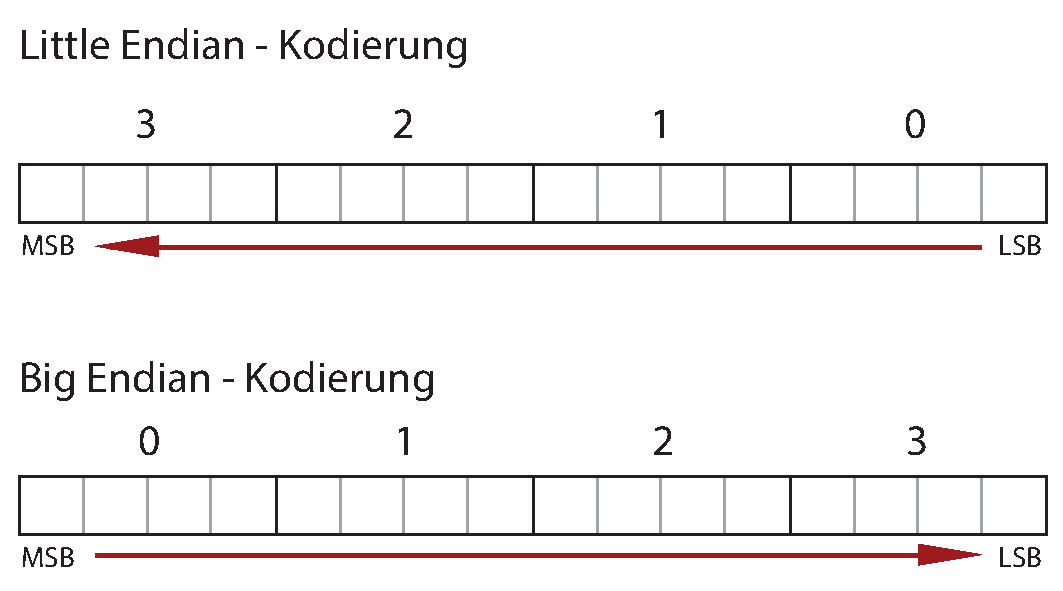
\includegraphics[angle=0,width=10cm]{./img/byteorder.pdf}
  %\floatfoot{Vorlage für diese Darstellung ist die Grafik in \cite[A.1.2]{dicom:iod}}
  \caption{Kodierungsreihenfolge von 4 Byte bei Little Endian- und Big Endian-Darstellung}
  \label{byteorder}
  \vspace{0.5cm}
\end{figure}

BitsStored gibt darüber Auskunft, wie viel Bit pro Wert in Anspruch genommen werden. Schließlich gibt HighBit das in der Reihenfolge ranghöchste Bit von StoredBits an \cite[8.1.1]{dicom:structure}.\\
Abbildung \ref{bits:pixel} verdeutlicht die Repräsentation eines Pixels im Datenelement PixelData. Die Darstellung entspricht einem eindimensionalen Array. Das erste Element ist das erste Pixel in der linken oberen Ecke, das letzte Element stellt den Pixel rechts unten dar. \ref{bits:16} und \ref{bits:8} zeigen die exakte Belegung an Bit bei BitsStored 16 und BitsStored 8. Der graue Hintergrund zeigt die allokierten Bit, während der rote Bereich den tatsächlich benutzten Speicher markiert. Der Pixelwert in Abbildung \ref{bits:8} nimmt den gesamten Speicherplatz pro Pixel ein. Das schwarze Quadrat steht für das HighBit.\\
Das Intervall der Werte ist abhängig von der Anzahl an gespeicherten Bits. Hat das Element StoredBits den Wert 12 kann ein  Pixel einen Wert aus dem Bereich von $[0, 2^{12}-1]$ annehmen. Entspricht StoredBits 8 ist das Intervall $[0, 2^8-1]$. Hier spricht man von einer Grauwerttiefe von 12 beziehungsweise 8 \cite[2.2]{handels:mbv}.
\begin{figure*}[htb]
%\subfigure[Keypoints]{\includegraphics[width=0.49\textwidth]{./img/basmati_keypoints.png}}\hfill
\centering
\fbox{
\subfigure[Pixel im Speicher]{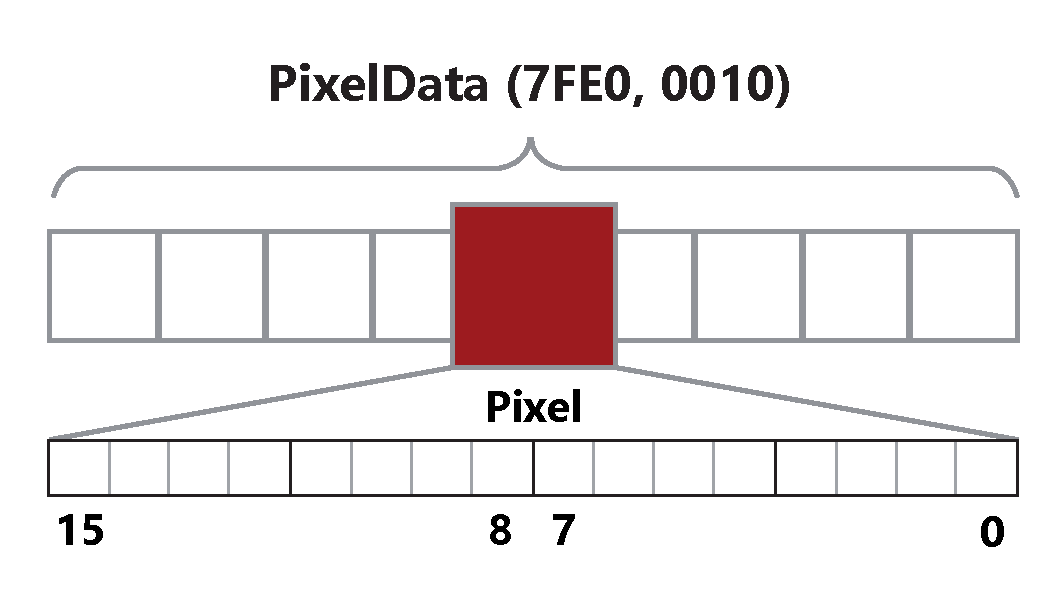
\includegraphics[width=5cm]{./img/bits.pdf} \label{bits:pixel}}
\subfigure[BitsAllocated 16, BitsStored 12, HighBit 11]{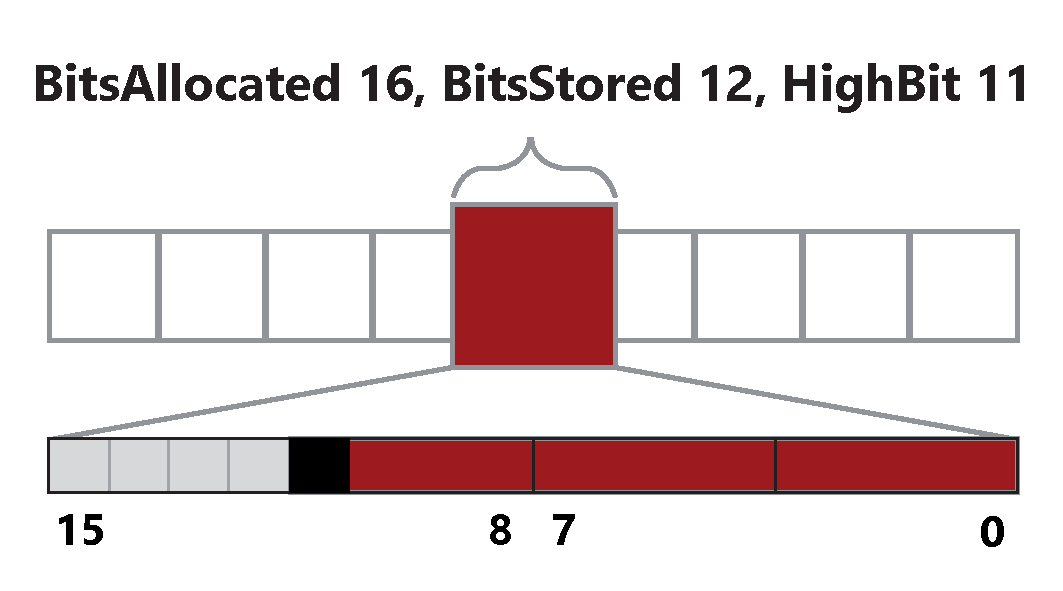
\includegraphics[width=5cm]{./img/bits16.pdf} \label{bits:16}}
\subfigure[BitsAllocated 8, BitsStored 8, HighBit 7]{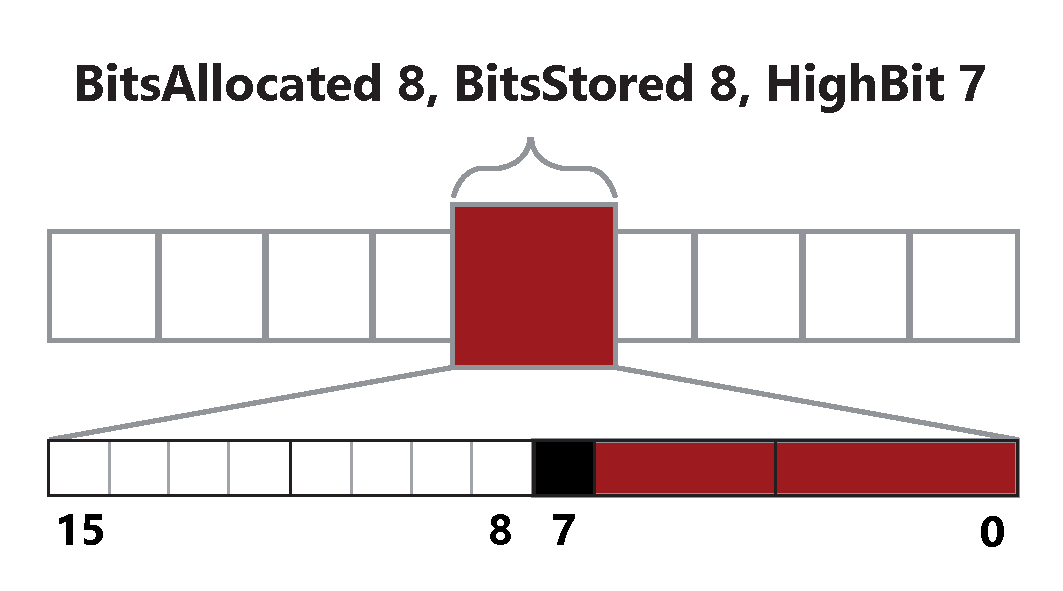
\includegraphics[width=5cm]{./img/bits8.pdf} \label{bits:8}}
}
\caption{Beispiele unterschiedlicher Speicherbelegung}
\label{bits}
\end{figure*}

Verschiedene Datenelemente aus dem DICOM-Standard liefern nähere Informationen zum Bildformat. So gibt das Element SamplesPerPixel (0028,0002) Auskunft darüber, wieviel Teile aus PixelData ein einzelnes Pixel repräsentieren. Hat Samples den Wert 1, so ist jedes Element aus PixelData genau ein Pixel. Daraus folgt, dass ein Grauwertbild vorliegt. 3 bedeutet, dass im DICOM-Objekt ein Farbbild mit den drei Kanälen rot, grün und blau liegt.\\
Die Werte der Pixel sind stark abhängig vom medizinischen Gerät, welches die Bilder aufzeichnet. Ein direkter Vergleich von Bildern, die von unterschiedlichen Geräten einer Modalität aufgezeichnet wurden ist daher nicht möglich. Um Gewebestrukturen von beispielsweise CT-Aufnahmen trotz dieser Abhängigkeiten patienten- und geräteübergreifend zu vergleichen, gibt es unter Anderem die Hounsfield Skala \cite[2.1.3]{handels:mbv}. Mit Hilfe der Datenelemente RescaleSlope und RescaleIntercept lassen sich die ursprünglichen Werte in brauch- und lesbare Pixelwerte konvertieren. RescaleType gibt die Skala an, mit der das Ergebnis interpretiert werden kann. Ein Umrechnung erfolgt mit der Formel aus \cite[C.11-1b Seite 1168]{dicom:iod}\\

\begin{equation}
Output=m*SV+b
\label{rescale}
\end{equation}

mit $m = RescaleSlope$, $b = RescaleIntercept$ und $SV=Pixelwert$.

Fettgewebe zum Beispiel nimmt nach der Hounsfield-Skala Werte zwischen 0 und -100 ein \cite[Abbildung 1.18 Seite 15]{radio:hounsfield}. Ob in einem DICOM-Objekt vorzeichenbehaftete Werte vorhanden sind, sagt das Element PixelRepresentation. Eine 0 bedeutet kein Vorzeichen. Bei einem Wert von 1 können negative Werte enthalten sein.
\begin{table}
    \begin{tabularx}{\textwidth}{|X|X|X|}
    \toprule
    \hline
    \textbf{Tag}         & \textbf{Tagname}     & \textbf{VR} \\ \hline
    (0028,0010) 		 & Rows					& US 		  \\ \hline
    (0028,0011) 		 & Columns				& US 		  \\ \hline
    (0028,0100) 		 & BitsAllocated		& US 		  \\ \hline
    (0028,0101) 		 & BitsStored			& US 		  \\ \hline
    (0028,0102)			 & HighBit				& US 		  \\ \hline
    \bottomrule
    \end{tabularx}
    \caption {Grundlegende Datenelemende für die digitale Repräsentation}
    \label{table:digitalRep}
\end{table}

\subsection{Grauwertbilder} \label{grey_images}

Für Bildverarbeitungsprozesse und Algorithmen bieten Grauwertbilder einige Vorteile im Vergleich zu Farbbildern. Der größte Unterschied liegt beim Verhältnis zwischen Informationsgehalt zu Speicherbedarf. Farben bieten bei Kantenübergängen oder Helligkeitsinformationen keinen Mehrwert. Das führt unter Anderem dazu, dass Industrie oder auch die medizinische Bildverarbeitung vorwiegend auf dieses Format zurückgreifen.\\
Eine Grauwerttiefe von 8 Bit ist Standard in der Bildverarbeitung. Das entspricht dem Intervall von $[0,255]$ und den Werten, die mit handelsüblichen Monitoren darstellbar sind. Medizinische Bilddaten können, wie in Abschnitt \ref{pixelkodierung} beschrieben, eine Tiefe von bis zu 16 Bit annehmen und Grauwerte aus dem Bereich $[0,65535]$ repräsentieren.

\begin{figure*}[htb]
%\subfigure[Keypoints]{\includegraphics[width=0.49\textwidth]{./img/basmati_keypoints.png}}\hfill
\centering
\fbox{
\subfigure[CT]{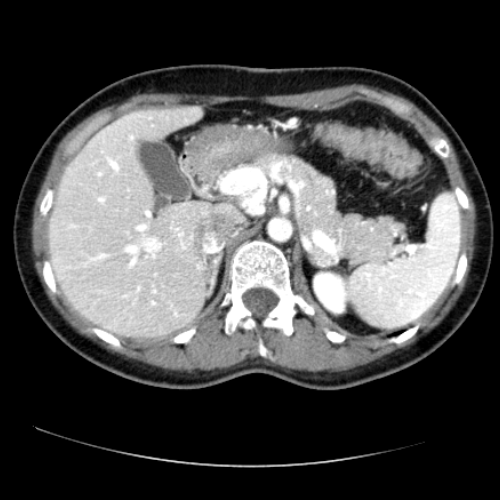
\includegraphics[width=5cm]{./img/ct.png} \label{ct}}
\subfigure[MR]{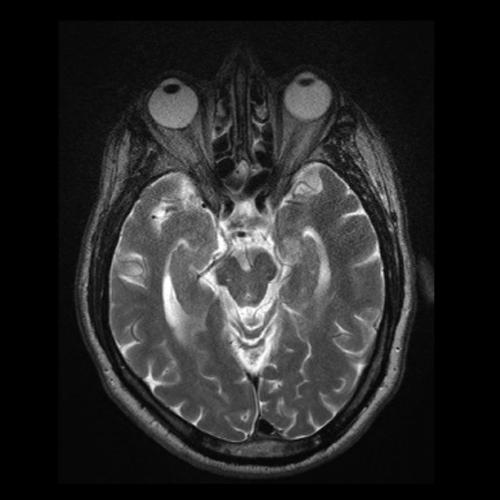
\includegraphics[width=5cm]{./img/mr.png} \label{mr}}
\subfigure[Ultraschall]{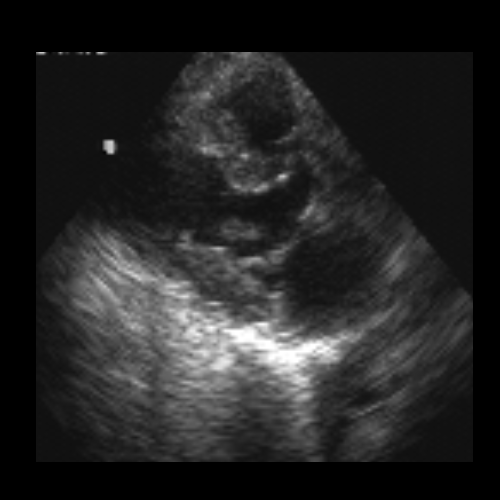
\includegraphics[width=5cm]{./img/sono.png} \label{sono}}
}
\floatfoot{Die Beispieldaten stammen von http://www.osirix-viewer.com/datasets/ - abgerufen am 19.01.2014}
\caption{Verschieden Graustufenbilder}
\label{grey}
\end{figure*}

\subsubsection{Fensterung von Grauwerten} \label{windowing}

Wie bereits in \ref{grey_images} beschrieben, lassen sich auf üblichen Monitoren nicht alle Grauwerte zur gleichen Zeit anzeigen. Dadurch müssen die maximal 65535 verschiedenen Grauwerte auf 255 abgebildet werden können. Dies wird durch die in der Radiologie verwendete Fensterungstechnik möglich\cite[Kapitel 8, Seite 249]{handels:mbv}. Es wird ein Fensterzentrum und eine Fensterbreite gewählt. Alle Werte innerhalb dieses Intervalls werden zwischen 0 und 255 umgerechnet. Abbildung \ref{window_graph} verdeutlicht dieses Prinzip. Ein CT-Bild mit einer Tiefe von 12 Bit besitzt 4096 Grauwerte. Ein Zentrum von 2000 und eine Breite von 500 bildet alle Werte von 1750 bis 2250 auf 0 bis 255 ab. Ist ein Pixeldatum kleiner 1750 wird das Minimum 0 hinterlegt und ist der Wert größer 2250 bekommt das Pixel das Maximum 255.\\
Im DICOM-Standard ist ein Algorithmus gegeben, um die Pixeldaten zu konvertieren\cite[C.11.2.1.2]{dicom:iod}.

\begin{algorithm}
\caption{Berechne den Fensterungswert aus originalem Pixelwert}
\begin{algorithmic}[1] 
\STATE $X \leftarrow input$ - tatsächlicher Pixelwert
\STATE $Y \leftarrow output$ - konvertierter Wert zwischen 0 und 255
\STATE $C \leftarrow windowCenter$
\STATE $W \leftarrow windowWidth$
\IF{$X <= C - 0.5 - (W-1)/2$}
	\STATE  $Y = Y_{min}$
\ELSIF {$X > C - 0.5 + (W-1)/2$}
	\STATE $Y = Y_{max}$
\ELSE
	\STATE $Y = ((X-(C-0.5)) / (W-1)+0.5)*(Y_{max}-Y_{min})+Y_{min}$
\ENDIF
\end{algorithmic}
\end{algorithm}


\begin{figure*}[htb]
%\subfigure[Keypoints]{\includegraphics[width=0.49\textwidth]{./img/basmati_keypoints.png}}\hfill
\centering
\fbox{
\subfigure[Fensterungstechnik]{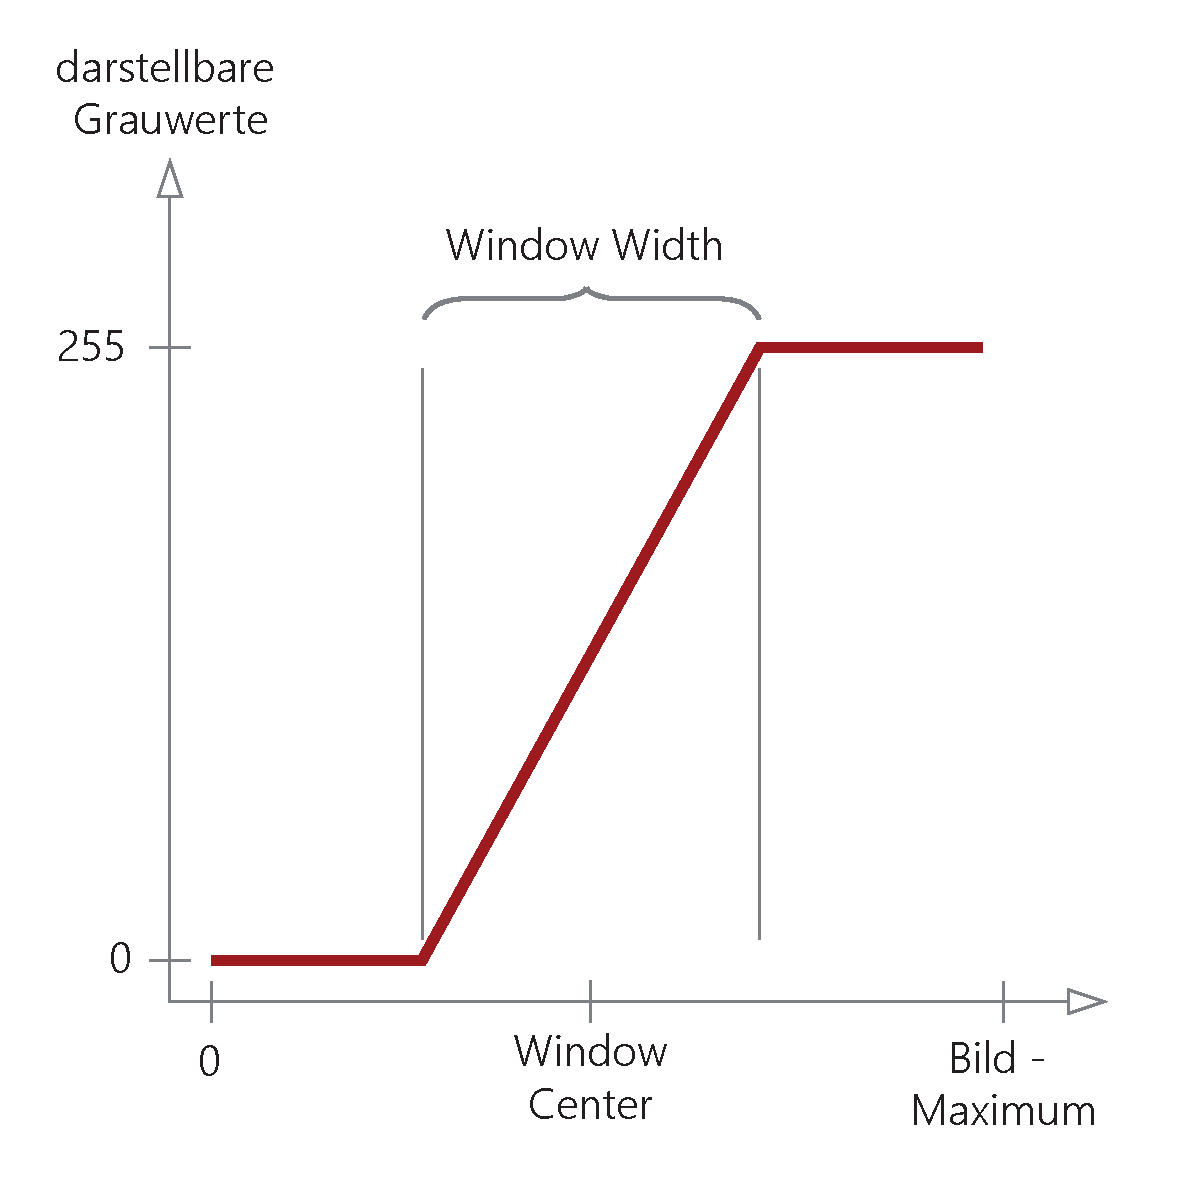
\includegraphics[width=5cm]{./img/fensterung.pdf} \label{window_graph}}
\subfigure[Window Center 50; Window Width 350]{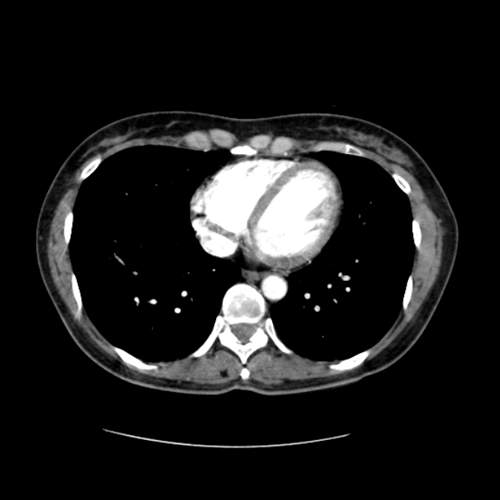
\includegraphics[width=5cm]{./img/window_a.png} \label{window_a}}
\subfigure[Window Center -124; Window Width 3134]{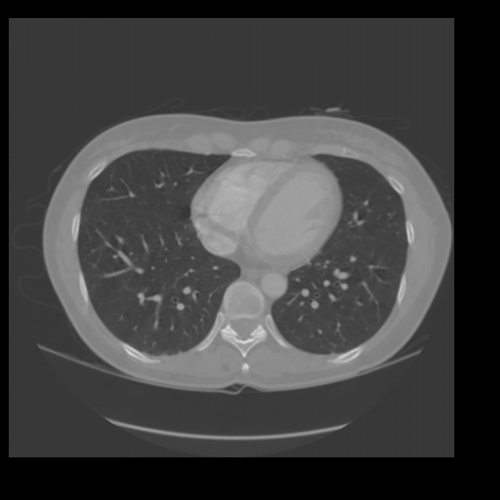
\includegraphics[width=5cm]{./img/window_b.png} \label{window_b}}
}
\floatfoot{Vorlage für die Grafik der Fensterungstechnik ist\cite[Abbildung 8.1]{handels:mbv}; Die Beispieldaten stammen von http://www.osirix-viewer.com/datasets/ - abgerufen am 19.01.2014}
\caption{Fensterungstechnik zur Darstellung medizinischer Bilddaten am handelsüblichen Monitor}
\label{window_sub}
\end{figure*}

\subsection{Farbbilder} \label{color_images}
Obwohl Grauwertbilder das am meisten verwendete Format in der medizinischen Bildverarbeitung darstellen, haben auch Farbbilder die verschiedensten Einsatzgebiete. So wird in der Dermatologie auf Farbdarstellungen zurückgegriffen um Hauterkrankungen zu dokumentieren\cite[2.2.3.2]{handels:mbv}. Des weiteren kann mit Farbultraschallbildern die Fließrichtung und Geschwindigkeit des Blutes visualisiert werden und dienen zur Untersuchung von Venen und Arterien\footnote{http://www.diagnostikum-berlin.de/farbkodierte-duplexsonographie-fkds - abgerufen am 19.01.2014}.\\
Wie bereits beschrieben, ist das Datenelement SamplesPerPixel mit einem Wert von drei der Indikator, dass ein Farbbild vorliegt. Das bedeutet pro Pixel werden 3 Elemente von PixelData belegt mit je einem Element für den roten, grünen und blauen Farbkanal. Daraus resultiert der dreifach Speicherbedarf, $BitsAllocated * SamplesPerPixel$ \cite[C.7.6.3.1.1]{dicom:iod}. Der DICOM-Standard bietet zwei Möglichkeiten, wie diese Information im Speicher hinterlegt werden. Entweder werden die Pixelwerte fortlaufend gespeichert mit R1, G1, B1; R2 ,G2, B2; ...RN, GN, BN; oder nach dem Kanal R1, R2, ...RN; G1, G2, ...GN; B1, B2, ...BN \cite[C.7.6.3.1.3]{dicom:iod}. Das Element dazu aus dem Data Dictionary heißt PlanarConfiguration(0028,0006). Abbildung \ref{planar} macht die beiden Schemata deutlich.

\begin{figure*}[htb]
%\subfigure[Keypoints]{\includegraphics[width=0.49\textwidth]{./img/basmati_keypoints.png}}\hfill
\centering
\fbox{
\subfigure[PlanarConfiguration = 0]{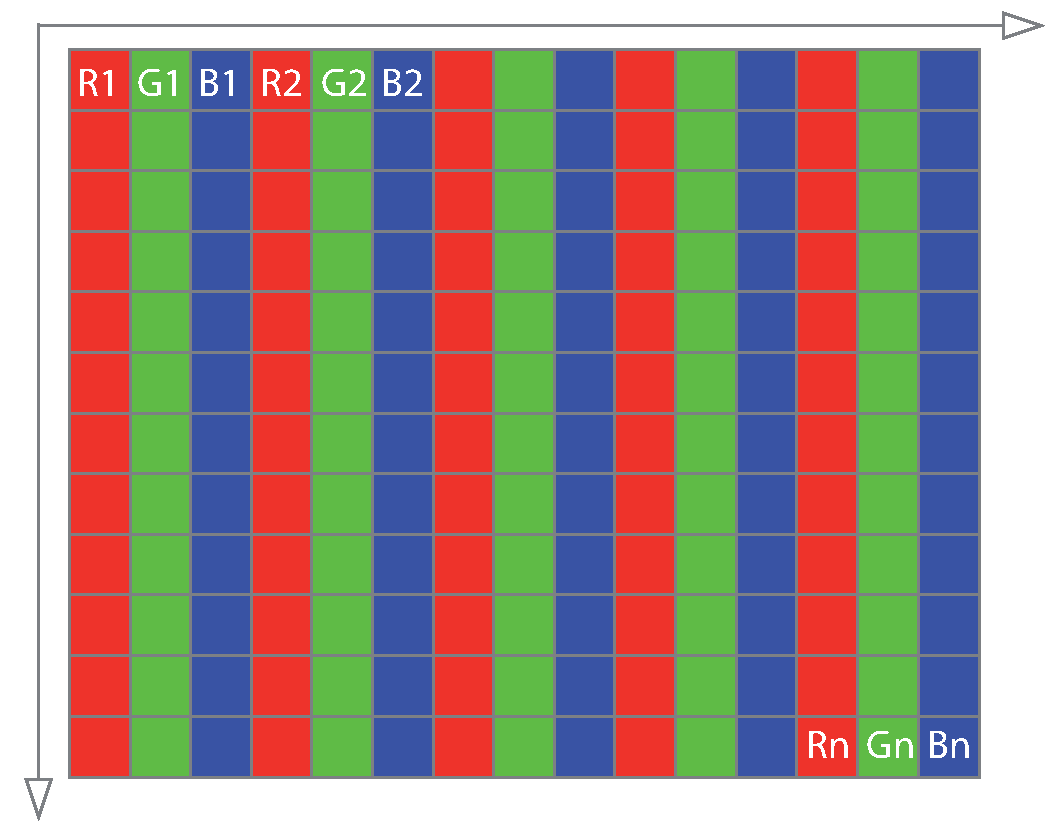
\includegraphics[width=8cm]{./img/planar_b.pdf} \label{planar_a}}
\subfigure[PlanarConfiguration = 1]{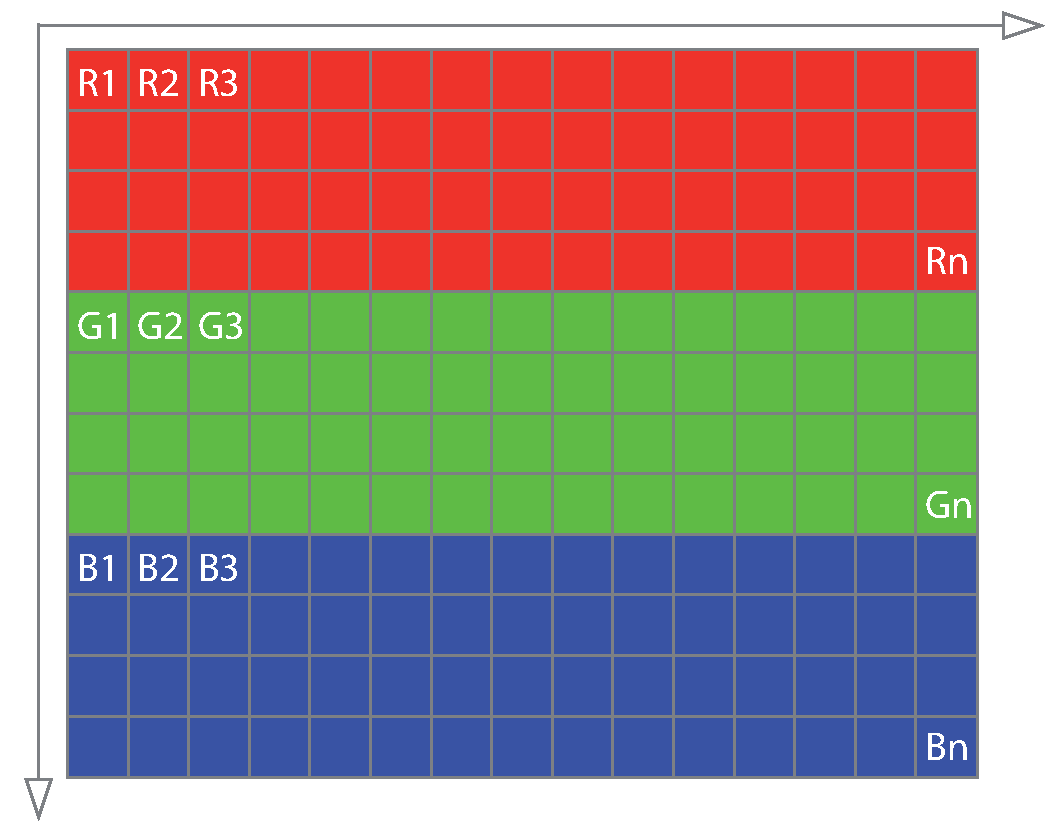
\includegraphics[width=8cm]{./img/planar_a.pdf} \label{plaanr_b}}
}
%\floatfoot{Vorlage für die Grafik der Fensterungstechnik ist\cite[Abbildung 8.1]{handels:mbv}; Die Beispieldaten stammen von http://www.osirix-viewer.com/datasets/ - abgerufen am 19.01.2014}
\caption{Kodierung der RGB-Werte im Datenelement PixelData mit Hilfe der PlanarConfiguration}
\label{planar}
\end{figure*}

\section{3D Bilddaten}
Sowohl die Grauwertdarstellungen, als auch Farbbilder wurden bisher nur als eine zweidimensionale Abbildung behandelt. Computertomographen und Magnetresonanztomographen sind in der Lage Schichten des menschlichen Körpers aufzunehmen. Die Menge der Schichtaufnahmen stellen eine Serie dar (vgl.\nameref{grundlagen:iod} \pageref{grundlagen:iod}). Durch die Verbindung der einzelnen DICOM-Objekte wird der Pixelraum verlassen und der Voxelraum betreten. Ein Voxel ist die dreidimensionale Repräsentation eines Pixels, mit der Tiefe als zusätzliche Dimension zu Breite und Höhe.

\begin{figure*}[htb]
%\subfigure[Keypoints]{\includegraphics[width=0.49\textwidth]{./img/basmati_keypoints.png}}\hfill
\centering
\fbox{
\subfigure[2D Darstellung]{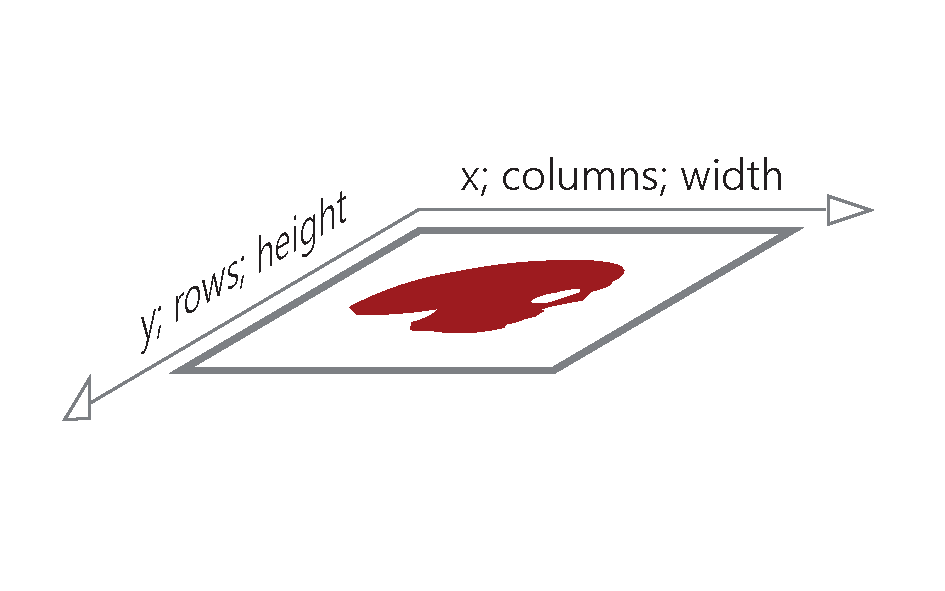
\includegraphics[width=5cm]{./img/2d.pdf} \label{2d}}
\subfigure[3D Bildfolge]{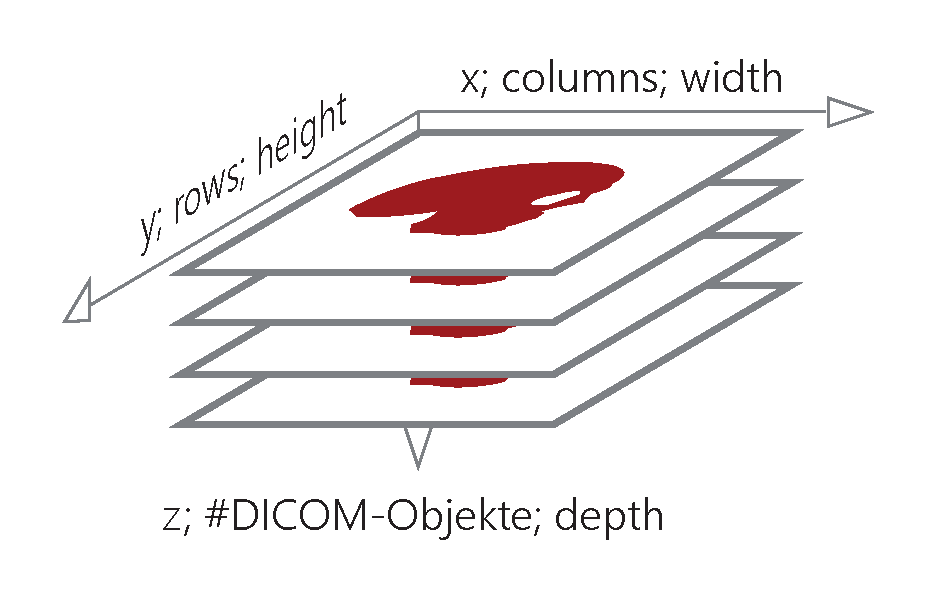
\includegraphics[width=5cm]{./img/3d.pdf} \label{3d}}
\subfigure[zeitlich Abhängige 3D Bildfolge]{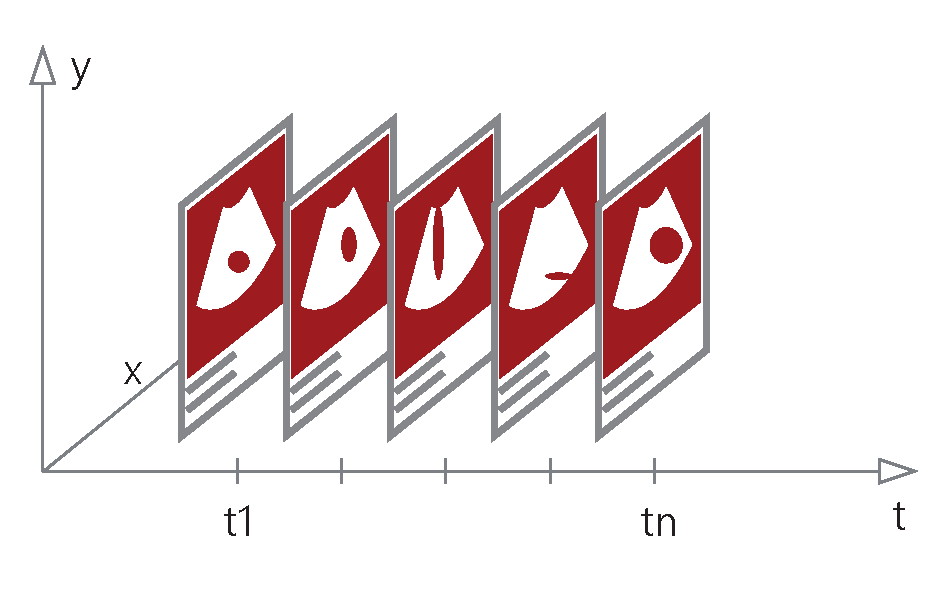
\includegraphics[width=5cm]{./img/time.pdf} \label{time3d}}
}
%\floatfoot{Vorlage für die Grafik der Fensterungstechnik ist\cite[Abbildung 8.1]{handels:mbv}; Die Beispieldaten stammen von http://www.osirix-viewer.com/datasets/ - abgerufen am 19.01.2014}
\caption{Darstellung von 2- und 3-dimensionalen Bilddaten}
\label{dimensions}
\end{figure*}

\section{Bilder mit zeitlicher Abhängigkeit}

Auch Bildaufnahmen zu verschiedenen Zeitpunkten sind dreidimensionale Bildfolgen, wobei die Zeit die dritte Dimension darstellt\cite[2.2.5]{handels:mbv}. Häufige Einsatzgebiete für Bewegtbildfolgen ist die Endoskopie oder Sonographie. Die Abbildung \ref{time3d} macht den Unterschied zwischen zeitlicher und räumlicher Dimension deutlich. Räumliche Darstellungen sind grundsätzlich in mehrere DICOM-Objekte und Dateien aufgeteilt. Zeitlich abhängige Daten sind in einem einzigen Objekt zusammengefasst. NumberOfFrames (0028,0008) gibt die Anzahl an unterschiedlichen Aufnahmen und Zeitpunkten an, die in PixelData enthalten sind.